\section{Method} \label{sec: method}



\subsection{Overall Framework} \label{sec: overall framework}

\begin{figure}[t]
	\centering
	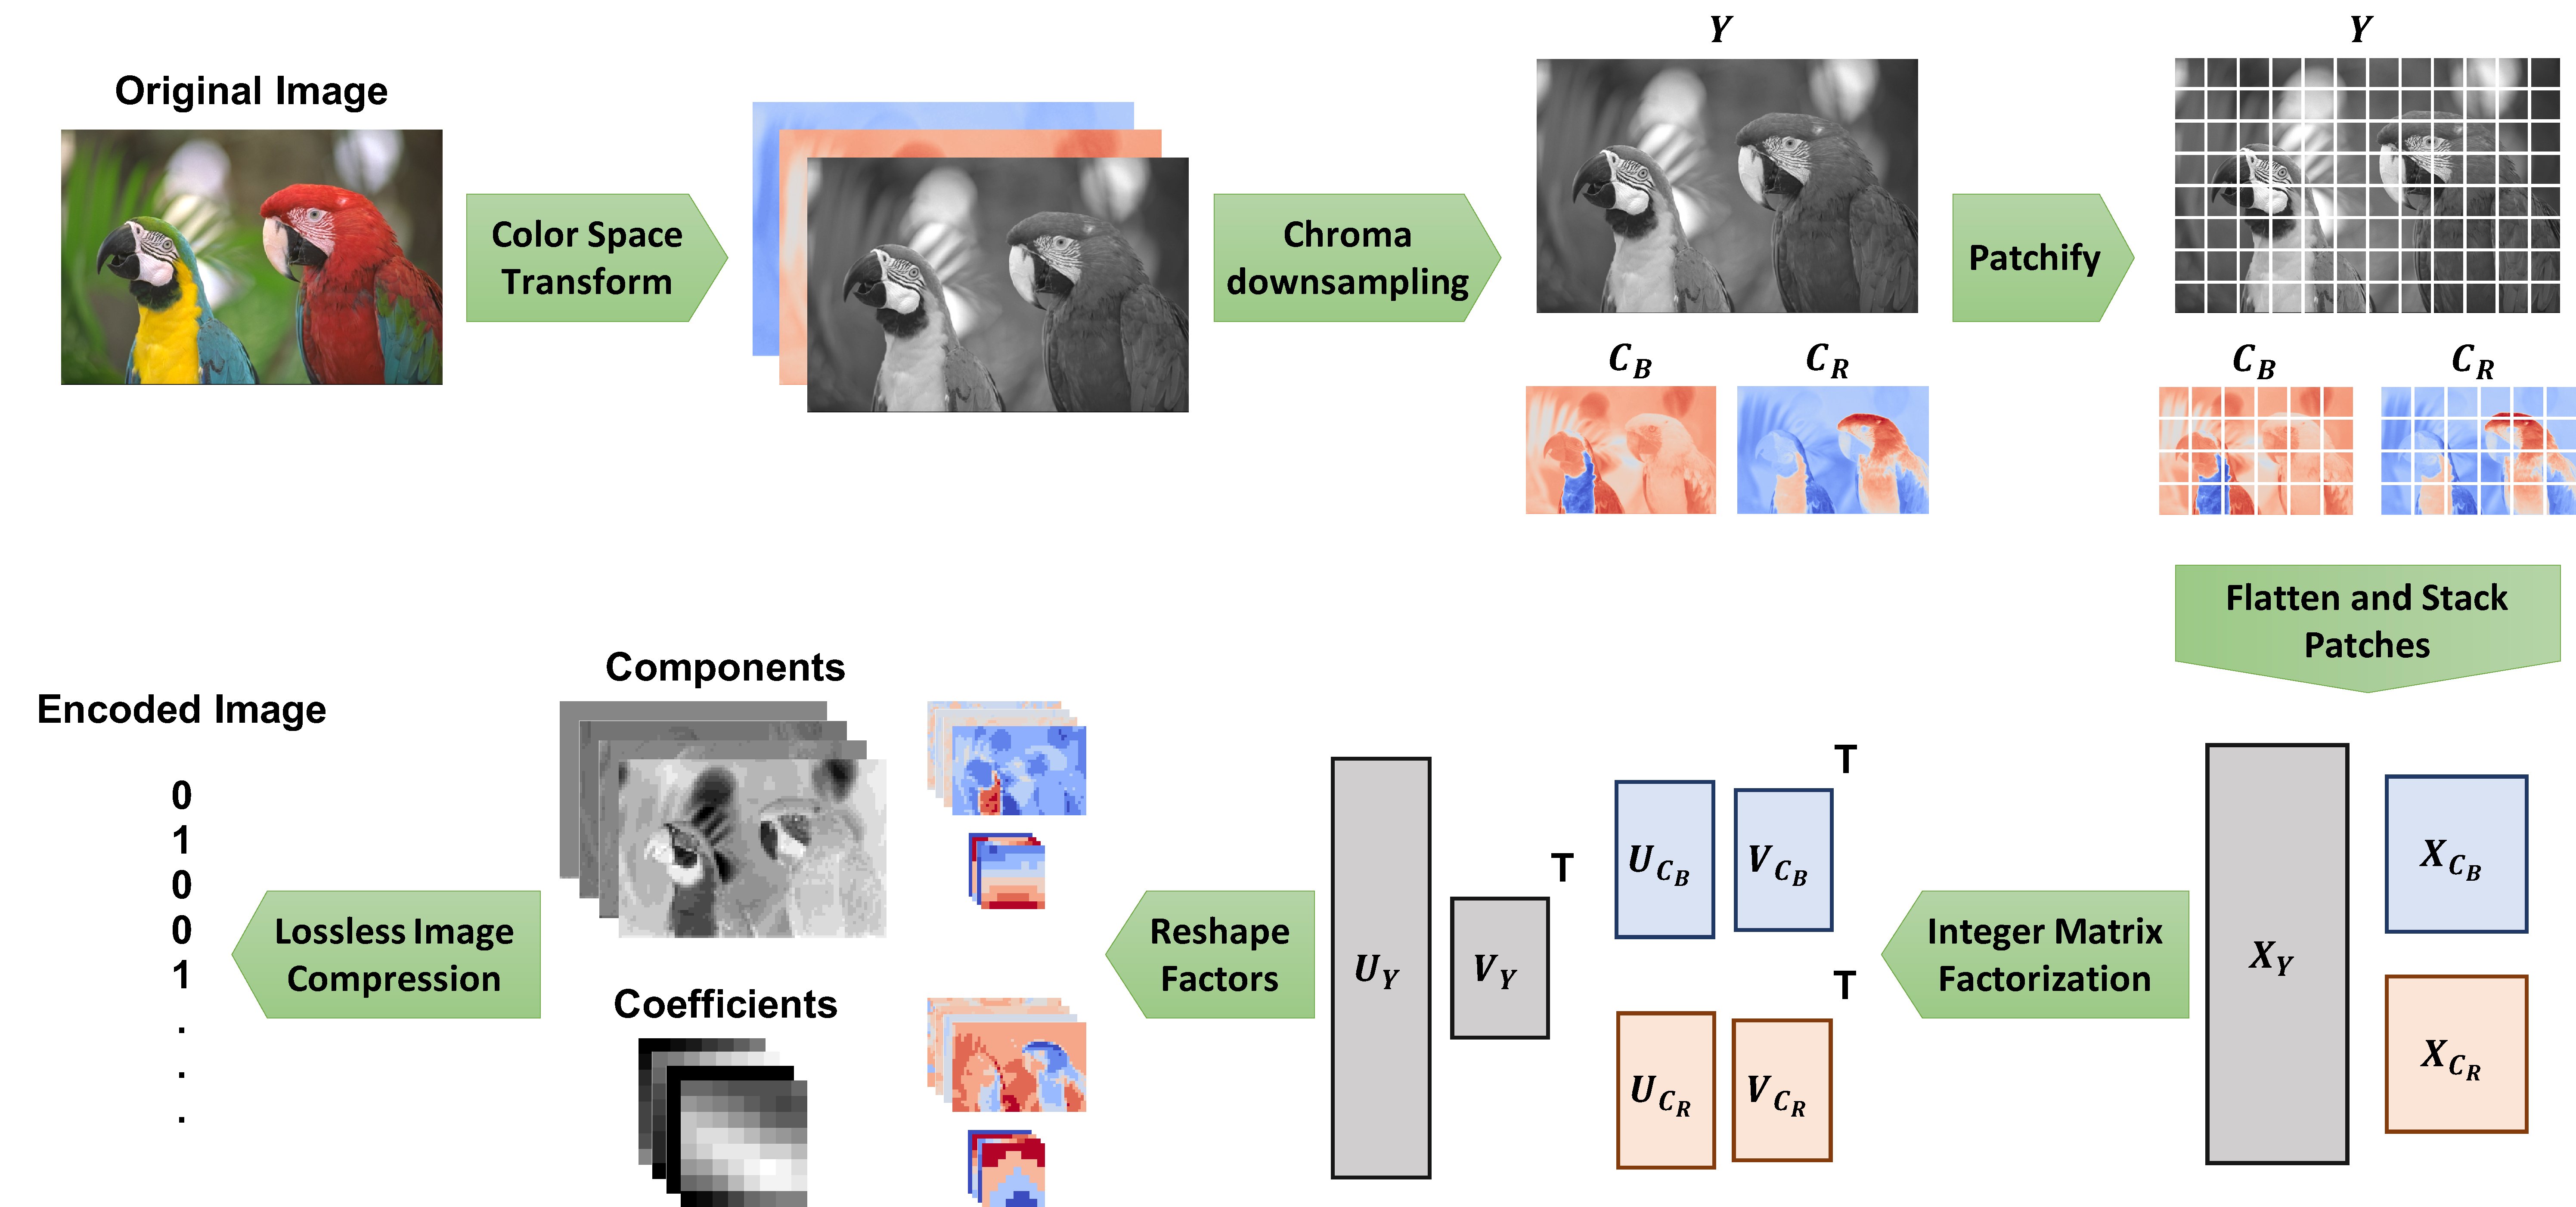
\includegraphics[width=\linewidth]{figures/imf_encoder.pdf}
	\vspace{10pt}
	\caption{An illustration of the encoder for our image compression method, based on integer matrix factorization.}
	\label{fig:imf_encoder}
\end{figure}

Figure \ref{fig:imf_encoder} illustrates an overview of the encoding pipeline for our proposed image compression method using integer matrix factorization (IMF). The encoder accepts an RGB image with dimensions $H \times W$ and a color depth of 8 bits, represented by the tensor $\bm{\mathcal{X}} \in \{0, \ldots, 255\}^{3 \times H \times W}$. Each step of encoding is described in the following.

\paragraph{Color Space Transformation.}
Analogous to the JPEG standard, the image is initially transformed into the YC\textsubscript{B}C\textsubscript{R} color space:
\begin{equation} \label{eq: ycbcr transform}
	\begin{bmatrix}
		Y \\
		C_B \\
		C_R
	\end{bmatrix} \triangleq
	\begin{bmatrix}
		0.299 & 0.587 & 0.114 \\
		-0.168736 & -0.331264 & 0.5 \\
		0.5 & -0.418688 & -0.081312
	\end{bmatrix}
	\begin{bmatrix}
		R \\
		G \\
		B
	\end{bmatrix}
	+
	\begin{bmatrix}
		0 \\
		128 \\
		128
	\end{bmatrix},
\end{equation}
where $Y$ represents the \emph{luma} component, and $C_B$ and $C_R$ are the blue-difference and red-difference \emph{chroma} components, respectively.  Note that as a result of this transformation, the elements of the luma ($\bm{Y}$) and chroma ($\bm{C}_B$, $\bm{C}_R$) matrices are no longer integers and can take any value within the range $[0, 255]$.

\paragraph{Chroma Downsampling.} 
After conversion to the YC\textsubscript{B}C\textsubscript{R} color space, the chroma channels $C_B$ and $C_R$ are downsampled by a factor of 2, similar to the process used in JPEG. This results in three components: the luma matrix $\bm{Y} \in [0, 255]^{H \times W}$ and the chroma matrices $\bm{C}_B, \bm{C}_R \in [0, 255]^{\frac{H}{2} \times \frac{W}{2}}$. This downsampling leverages the fact that the human visual system perceives far more detail in brightness information (luma) than in color saturation (chroma).

\paragraph{Patchification.} 
Each of the matrices $\bm{Y} \in [0, 255]^{H \times W}$, $\bm{C}_B \in [0, 255]^{\frac{H}{2} \times \frac{W}{2}}$, and $\bm{C}_R \in [0, 255]^{\frac{H}{2} \times \frac{W}{2}}$ is split into non-overlapping $8 \times 8$ patches. If a dimension of a matrix is not divisible by 8, the matrix is first padded to the nearest size divisible by 8 using reflection of the boundary values. These patches are then flattened into row vectors and stacked vertically to form matrices $\bm{X}_{Y} \in [0, 255]^{\frac{HW}{64} \times 64}$, $\bm{X}_{C_B} \in [0, 255]^{\frac{HW}{256} \times 64}$, and $\bm{X}_{C_R} \in [0, 255]^{\frac{HW}{256} \times 64}$. Later, these matrices will be low-rank approximated using integer matrix factorization (IMF). Note that this patchification technique differs from the block splitting in JPEG, where each block is subject to discrete cosine transform (DCT) and processed independently. The patchification technique not only captures the locality and spatial dependencies of neighboring pixels but also performs better with the matrix decomposition approach to image compression.

\paragraph{Low-rank approximation.} We can now low-rank approximate the matrices $\bm{X}_{Y}$, $\bm{X}_{C_B}$, $\bm{X}_{C_R}$, which is the core step in our compression method that provides a lossy compressed represention of these matrices. The low-rank approximation \citep{eckart1936approximation} seeks to approximate some given matrix $ \mathbf{X} \in \mathbb{R}^{M \times N} $ by 
\begin{equation} \label{eq: lra}
	\bm{X} \approx \bm{U} \bm{V}^\mathsf{T} = \sum_{r=1}^{R} U_{:r} {V_{:r}}^\mathsf{T},
\end{equation} 
where $\bm{U} \in \mathbb{R}^{M \times R}$ and $\bm{V} \in \mathbb{R}^{N \times R}$ are \emph{factor matrices}, and $R \leq \min(M,N)$ is known as the \emph{rank}. By setting $R$ to sufficiently small value, the factor matrices $\bm{U}$ and $\bm{V}$ with a combined number of $(M+N)R$ elements provide a compressed representation of the original matrix with $MN$ elements, encapsulating the most significant patterns in the image. With

\paragraph{Reshape factors.}


\paragraph{Lossless image compression.}



\subsection{Integer Matrix Factorization (IMF)} \label{sec: imf}



\subsection{Block Coordinate Descent Scheme for IMF} \label{sec: bcd}



\begin{theorem}  \label{the: bcd monotonicity}
The IMF cost function, $\| \bm{X} - \bm{U} \bm{V}^\mathsf{T} \|_\text{F}^2$, is monotonically nonincreasing under each of the multiplicative update rules.
\end{theorem}

\begin{proof}
See Appendix \ref{app: proof} for the proof.
\end{proof}


\subsection{Implementation Details} \label{sec: implementation details}